% Latex template: mahmoud.s.fahmy@students.kasralainy.edu.eg
% For more details: https://www.sharelatex.com/learn/Beamer

\documentclass[aspectratio=1610]{beamer}					% Document class

\setbeamertemplate{footline}[text line]{%
  \parbox{\linewidth}{\vspace*{-8pt}A brief introduction to graphical models and deep methods in computational network biology \hfill\insertshortauthor\hfill\insertpagenumber}}
\setbeamertemplate{navigation symbols}{}

\usepackage[english]{babel}				% Set language
\usepackage[utf8x]{inputenc}			% Set encoding

\mode<presentation>						% Set options
{
  \usetheme{default}					% Set theme
  \usecolortheme{default} 				% Set colors
  \usefonttheme{default}  				% Set font theme
  \setbeamertemplate{caption}[numbered]	% Set caption to be numbered
}

% Uncomment this to have the outline at the beginning of each section highlighted.
%\AtBeginSection[]
%{
%  \begin{frame}{Outline}
%    \tableofcontents[currentsection]
%  \end{frame}
%}

\usepackage{graphicx}					% For including figures
\usepackage{booktabs}					% For table rules
\usepackage{hyperref}					% For cross-referencing
\usepackage[absolute,overlay]{textpos}
\usepackage{bm}

\title{Linear Gene Networks}	% Presentation title
\author{Clayton W. Seitz}								% Presentation author
\date{\today}									% Today's date	

\begin{document}

% Title page
% This page includes the informations defined earlier including title, author/s, affiliation/s and the date
\begin{frame}
  \titlepage
\end{frame}

% Outline
% This page includes the outline (Table of content) of the presentation. All sections and subsections will appear in the outline by default.
\begin{frame}{Outline}
  \tableofcontents
\end{frame}

% The following is the most frequently used slide types in beamer
% The slide structure is as follows:
%
%\begin{frame}{<slide-title>}
%	<content>
%\end{frame}

\begin{frame}{Example gene regulatory network in yeast}

\begin{figure}
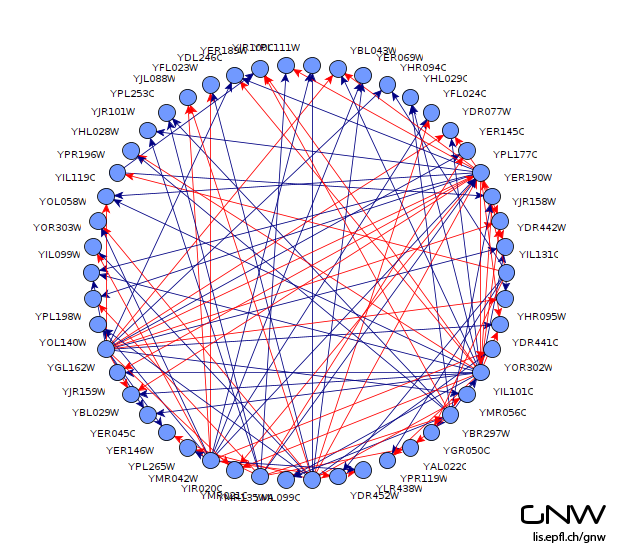
\includegraphics[width=9.5cm]{yeast-net.png}
\end{figure}

\end{frame}

\begin{frame}{Linear dynamics of transcription and translation}

\begin{textblock*}{15cm}(1cm,1.25cm)
Assumptions: gene-gene interactions are linear, noise is Gaussian, long protein lifetimes
\end{textblock*}

\begin{textblock*}{7cm}(0cm,1.75cm)
\begin{figure}
\begin{align*}
\dot{x_{i}} &= \sum_{j}m_{ji}y_{j} - \alpha_{i}x_{i} + \eta_{i}\\
\dot{y_{i}} &= r_{i}x_{i} - \beta_{i}y_{i} + \xi{i}
\end{align*}
\end{figure}
\end{textblock*}

\begin{textblock*}{7cm}(1cm,4.75cm)
If we assume that $\dot{y_{i}} \approx 0$ we have a Langevin equation for $x(t)$
\end{textblock*}

\begin{textblock*}{7cm}(7cm,1.75cm)
\begin{figure}
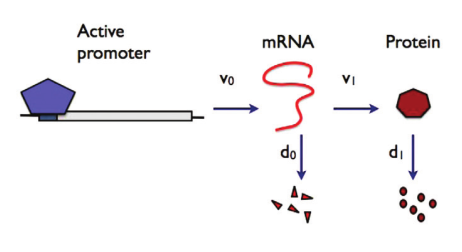
\includegraphics[width=7cm]{linear.png}
\end{figure}
\end{textblock*}

\begin{textblock*}{15cm}(1cm,6.5cm)

For example, a three-dimensional gene network:

\begin{equation*}
\begin{bmatrix} 
    \dot{x_{1}}\\
	\dot{x_{2}}\\
	\dot{x_{3}}\\
    \end{bmatrix}
    =
\begin{bmatrix} 
    -\alpha_{1} & m_{21} & m_{31} \\
	m_{12} & -\alpha_{2} & m_{32}\\
	m_{13} & m_{23} & -\alpha_{3} \\
\end{bmatrix}
\begin{bmatrix} 
    x_{1}\\
	x_{2}\\
	x_{3}\\
    \end{bmatrix}
+ 
\begin{bmatrix} 
    \eta_{1}\\
	\eta_{2}\\
	\eta_{3}\\
    \end{bmatrix}
\end{equation*}

\end{textblock*}

\end{frame}

\begin{frame}{Ornstein-Uhlenbeck process}

Existence of an equilibrium distribution

Gaussian distribution

Conditional distributions of multivariate Gaussian

\end{frame}

\begin{frame}{Bayesian network for a multivariate Gaussian}
\end{frame}

\begin{frame}{Bayesian inference of model parameters}
\end{frame}

\end{document}
